\chapter{\IfLanguageName{dutch}{Resultaten}{Resultaten}}
\label{ch:resultaten}
In dit hoofdstuk worden de testen en hun resultaten besproken.
\section{\IfLanguageName{dutch}{Bespreking requirementanalyse}{Analyzing requirementanalyse}}
In deze sectie worden de resultaten van de enquête besproken.
\newline
De bevraging bestaat slechts uit een kleine steekproef (n=70), omdat de enquête gericht is op een kleine populatie (water- en wintersporters). Uit de enquête blijkt dat de meeste correspondenten al gehoord hebben van een GPS-tracker (95,7\%). Ondanks velen ervan gehoord hebben, heeft slechts 28,6\% reeds overwogen om een GPS-tracker aan te schaffen. De ontwikkelde proof of concept is innovatiever, doordat het zeer makkelijk te tracken is aan de hand van een webapplicatie. Deze technologie is vrij onbekend bij de steekproef, want 42,9\% heeft nog nooit gehoord van zo een systeem. 
\newline
De prijs van de proof of concept (148 euro) wordt niet aanschouwt als budgettair. Uit de enquête (zie figuur:\ref{graph:price}) blijkt dat de correspondenten 148 euro teveel vinden voor een GPS-tracker. (mediaan = 75 euro, gemiddelde = 99,98 euro) 
\begin{figure}
	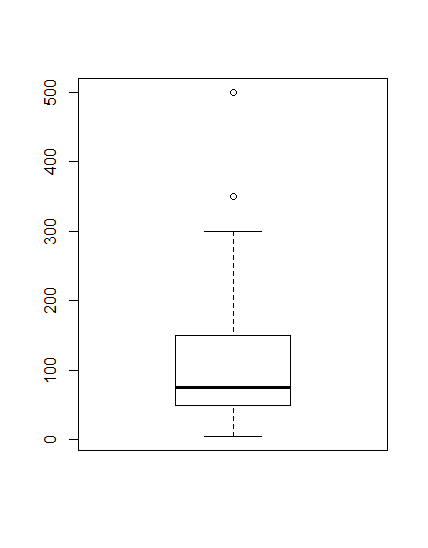
\includegraphics[width=\textwidth,height=\textheight,keepaspectratio]{boxplot_prices.png}
	\caption{Boxplot over de maximum prijs dat een correspondent wilt betalen voor een GPS-tracker}
	\label{graph:price}
\end{figure}
\newline
Wat opvallend is, is dat de waterdichtheid belangrijker is dan de accuraatheid. Zo scoort (uitgedrukt in gemiddelde, op 10) de waterdichtheid een 9,6 en de accurhaatheid van de lokatiebepaling slechts 8,5. De gebruiksvriendelijkheid scroort een 8,1. 
\newline
De batterijduur van de proof of concept voldoet aan de eisen van de correspondenten, namelijk 24 uur. De batterijduur kan ook verlengt worden indien er gebruik gemaakt wordt van een powerbank.
\newline
Indien de proof of concept op de markt komt, zou 28,6\% deze aanschaffen, ondanks de prijs hoger ligt dan gewenst. 54.3\% twijfelt nog. 
\newline
De proof of concept zou gebruikt worden voor:
\begin{itemize}
	\item watersport = 38,6\&
	\item sneeuwsport = 22,9\%
	\item water- en sneeuwsport = 38,6\%
\end{itemize}
\pagebreak
\section{\IfLanguageName{dutch}{Vergelijking tussen GPS van een gsm en proof of concept}{Difference between the GPS from a phone and the proof of concept}}
Tijdens de eerste test werden er 2 toestellen gebruikt: de proof of concept en een gsm. De gsm is een Xiaomi Mi 9T (kostprijs 332 euro).
Voor de eerste field test is er op voorhand een route uitgestippeld (zie figuur \ref{fig:uitgestippelde_route}). Tijdens het wandelen van deze route stuurde de proof of concept (\ref{ch:proof-of-concept}) en de mobiele applicatie (\ref{ch:mobileapp}) tegelijk hun locaties door met een tijdsinterval van telkens drie seconden. (Zie figuur \ref{fig:field_test_1})
\begin{figure}
	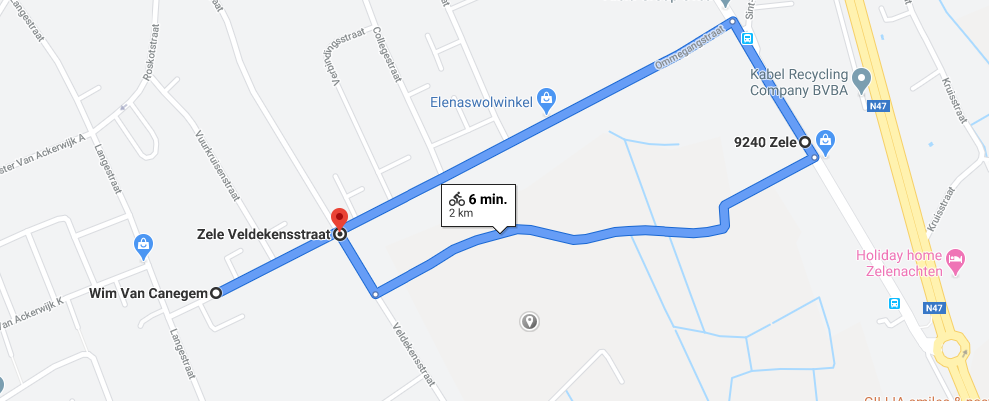
\includegraphics[width=\textwidth,height=\textheight,keepaspectratio]{uitgestippelde_route.png}
	\caption{De uitgestippelde route voor de eerste field test}
	\label{fig:uitgestippelde_route}
\end{figure}
\begin{figure}
	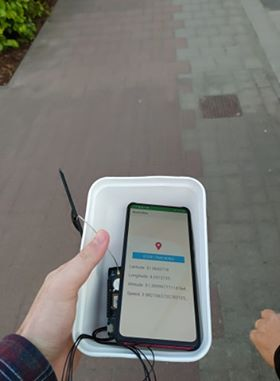
\includegraphics[width=50mm,height=100mm,keepaspectratio]{field_test_1.jpg}
	\caption{Het uitvoeren van de eerste field test}
	\label{fig:field_test_1}
\end{figure}
\newline
\newline
Het resultaat is zeer opmerkelijk. In figuur \ref{fig:field_test_1_resultaat} is het duidelijk dat de proof of concept (blauwe markers) beter scoort dan dan de GPS van een gsm (rode markers). Het is moeilijk om de exacte reden van deze discrepantie in resultaten te achterhalen, omdat de data van de GPS-chip alleen verkrijgbaar zijn voor de fabrikant. De enige data die verkregen kan worden van de GPS-chip is de berekende locatie. 
\newline
Het gebruik van Google Maps op een gsm kan een meer accurate lokatiebepaling doen in vergelijking met het resultaat van de field test. Dit komt omdat Android en iOS extra informatie gebruiken zoals gsm-masten en wifi signalen (SSIDs). Google Maps maakt ook gebruik van verschillende algoritmes om de locatie te schatten op een straat zodat deze accurater lijken.
\newline
Om de probleemstelling op te lossen, moet een GPS-tracker werken aan de kust en in berggebieden. Ook is de route niet op voorhand geweten, waardoor een gsm zeer slecht zou scoren als GPS-tracker omdat het geen gebruik kan maken van extra informatie en algoritmes van Google Maps. De proof of concept lijkt wel een goede oplossing te zijn voor de probleemstelling, omdat het volledig onafhankelijk is van extra informatie en/of algoritmes tijdens het gebruik van Google Maps. 
\newline
Uit de eerste field test kan er dus geconcludeerd worden dat de proof of concept slaagt in zijn opzet.
\begin{figure}
	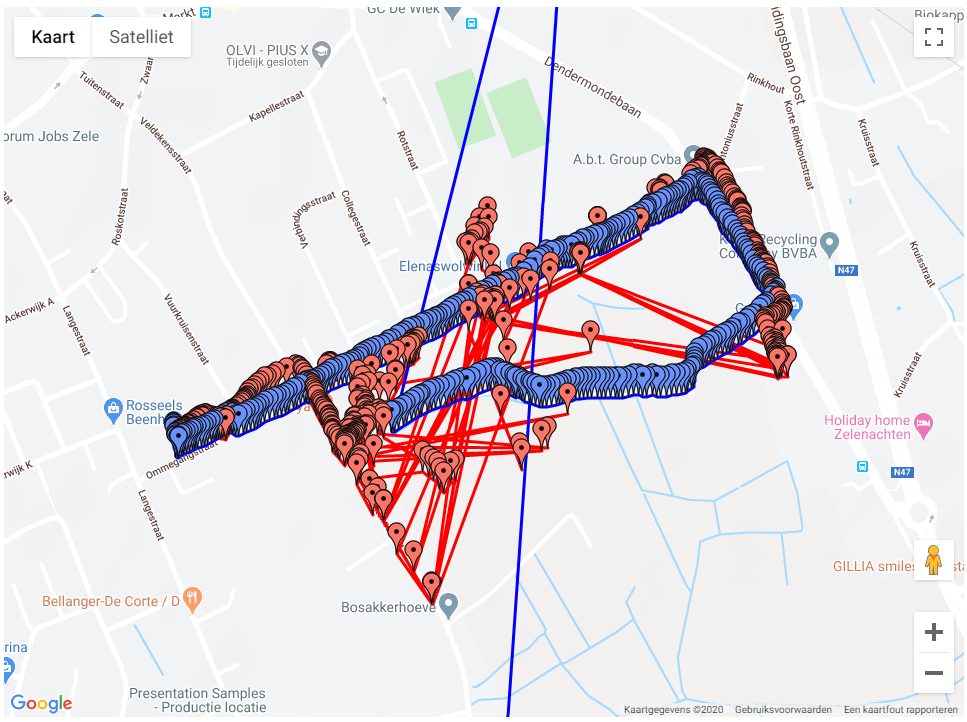
\includegraphics[width=\textwidth,height=\textheight,keepaspectratio]{field_test_1_resultaat.png}
	\caption{Resultaat van de eerste field test}
	\label{fig:field_test_1_resultaat}
\end{figure}